The predicted generated energy curves in Figures \ref{fig:plot:sub:mer-energy-production-predicted-vs-reported-my29-adjusted}, \ref{fig:plot:sub:mer-energy-production-predicted-vs-reported-my30-adjusted}, and \ref{fig:plot:sub:mer-energy-production-predicted-vs-reported-my32-adjusted} were obtained through the process described in Section \ref{sec:Appendix:NarrowedEnergyPredictionErrorMarginRange:PreservingOutliers}. This resulted in overly conservative predictions when compared with the curve representing energy productions reported by MER Opportunity.

Predictions in Figures \ref{fig:plot:sub:mer-energy-production-predicted-vs-reported-my29-adjusted-without-outliers}, \ref{fig:plot:sub:mer-energy-production-predicted-vs-reported-my30-adjusted-without-outliers}, and \ref{fig:plot:sub:mer-energy-production-predicted-vs-reported-my32-adjusted-without-outliers} were obtained through the process described in Section \ref{sec:Appendix:NarrowedEnergyPredictionErrorMarginRange:IgnoringOutliers}. This resulted in predictions that more closely follow reported energy productions. Comparing these predictions with the unadjusted ones presented in Figure \ref{fig:plot:mer-energy-production-predicted-vs-reported} shows little changes and therefor do not justify the need to narrow down the error margin range for the purposes of preliminary mission scenario analysis.

\begin{figure}[h]
\captionsetup[subfigure]{justification=centering}
\vspace{-2ex}
	\centering
    %% setup sizes
    \setlength{\subfigureWidth}{0.32\textwidth}
    \setlength{\graphicsHeight}{50mm}
    %% kill hyper-link highlighting
    \hypersetup{hidelinks=true}%
    %% the figures
	\begin{subfigure}[t]{\subfigureWidth}
        \centering
		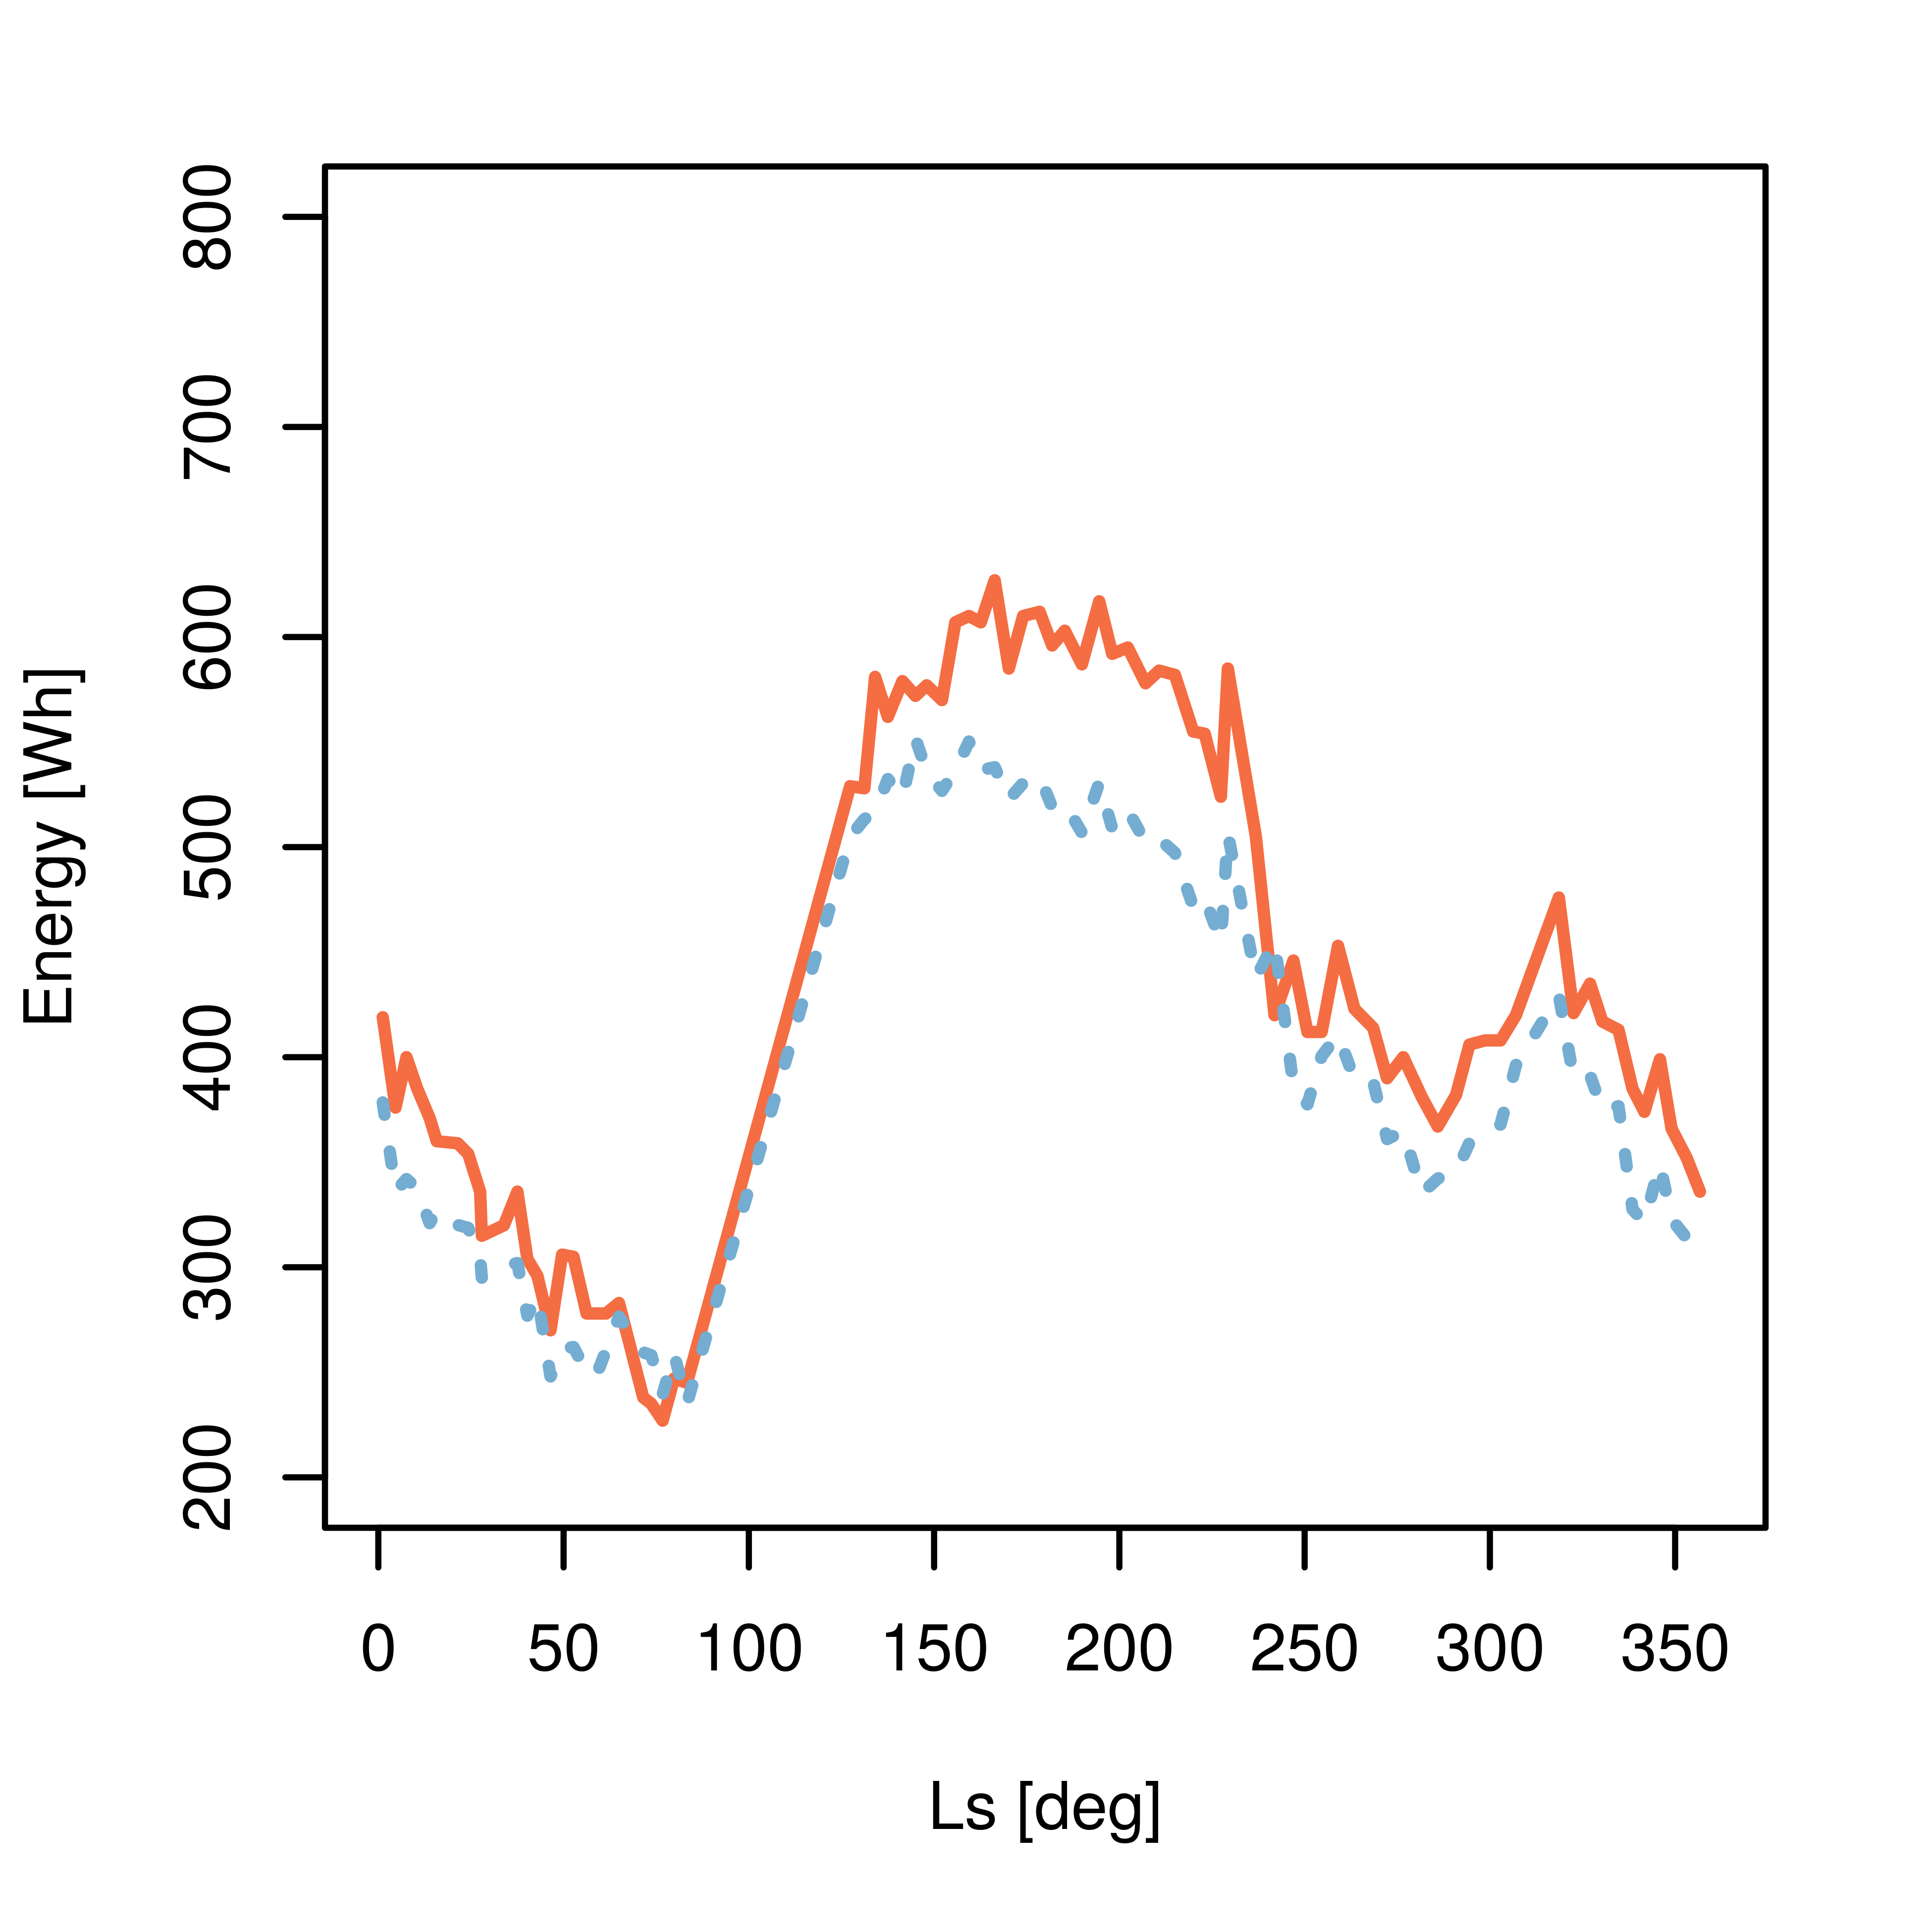
\includegraphics[height=\graphicsHeight]{sections/appendix/B/plots/predicted-vs-measured-energy-my29-adjusted.png}
		\subcaption{MY29}
		\label{fig:plot:sub:mer-energy-production-predicted-vs-reported-my29-adjusted}
	\end{subfigure}\hfill
	\begin{subfigure}[t]{\subfigureWidth}
        \centering
		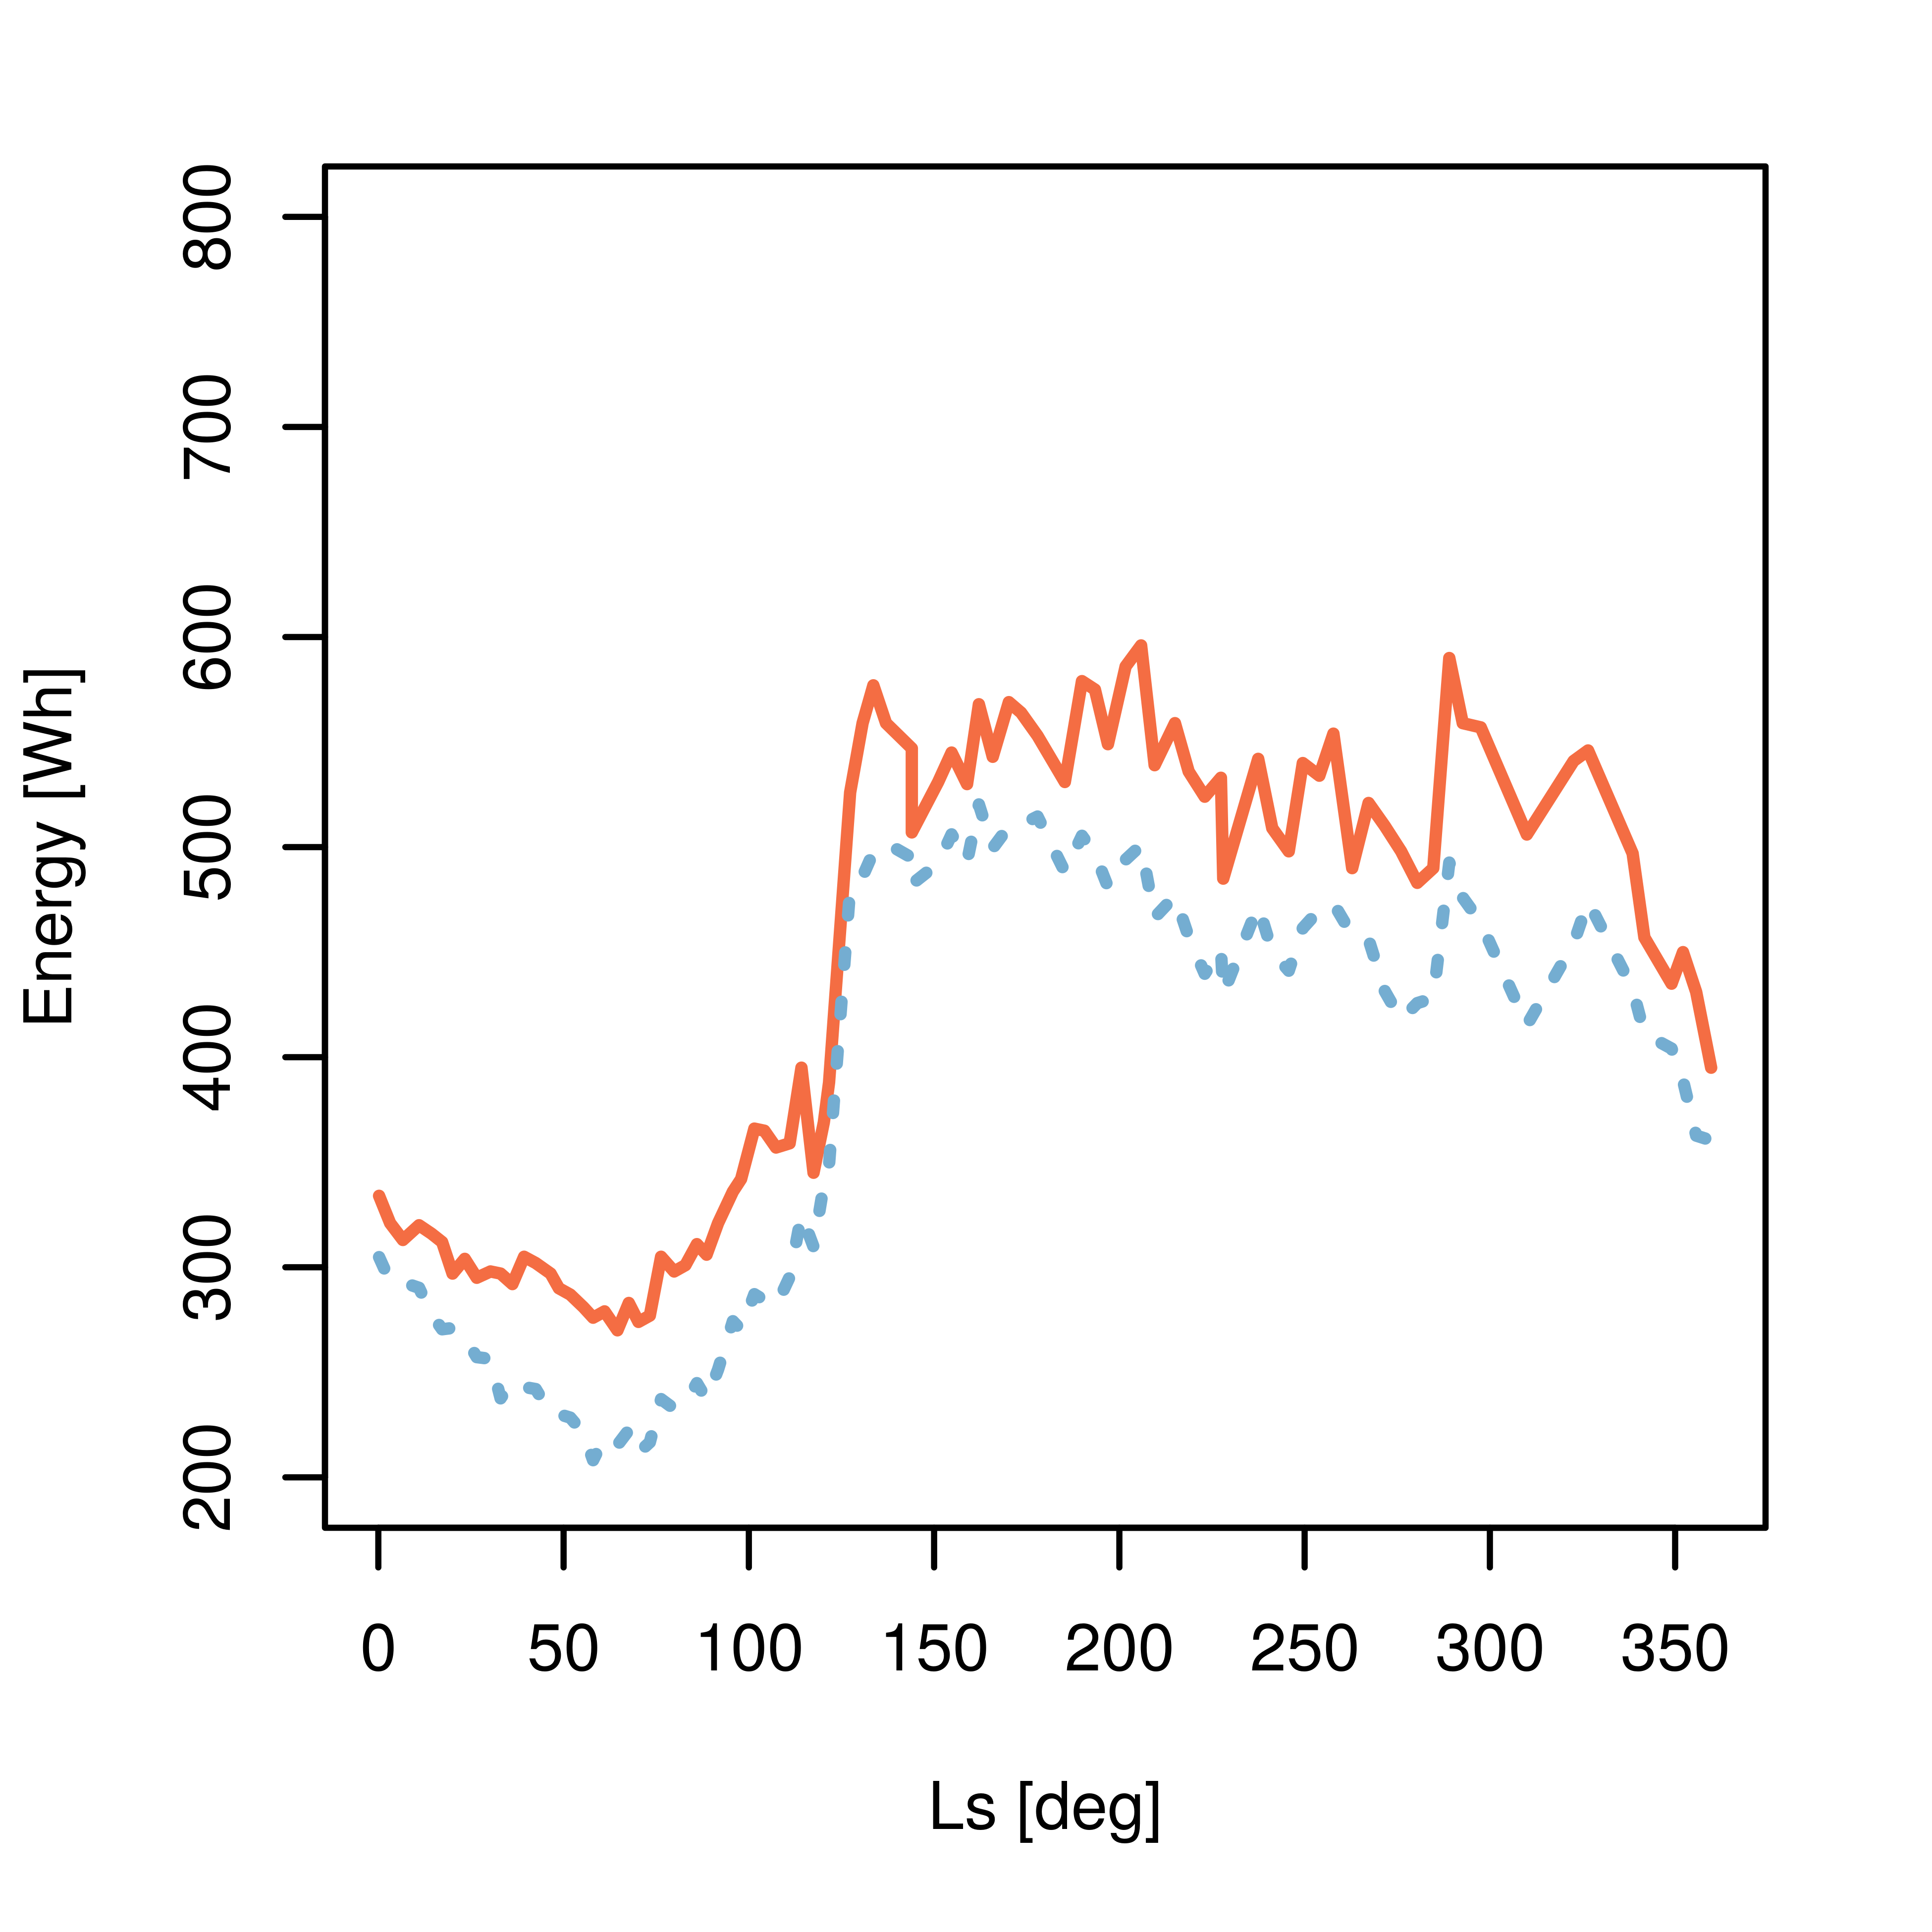
\includegraphics[height=\graphicsHeight]{sections/appendix/B/plots/predicted-vs-measured-energy-my30-adjusted.png}
		\subcaption{MY30}
		\label{fig:plot:sub:mer-energy-production-predicted-vs-reported-my30-adjusted}
	\end{subfigure}\hfill
    \begin{subfigure}[t]{\subfigureWidth}
        \centering
		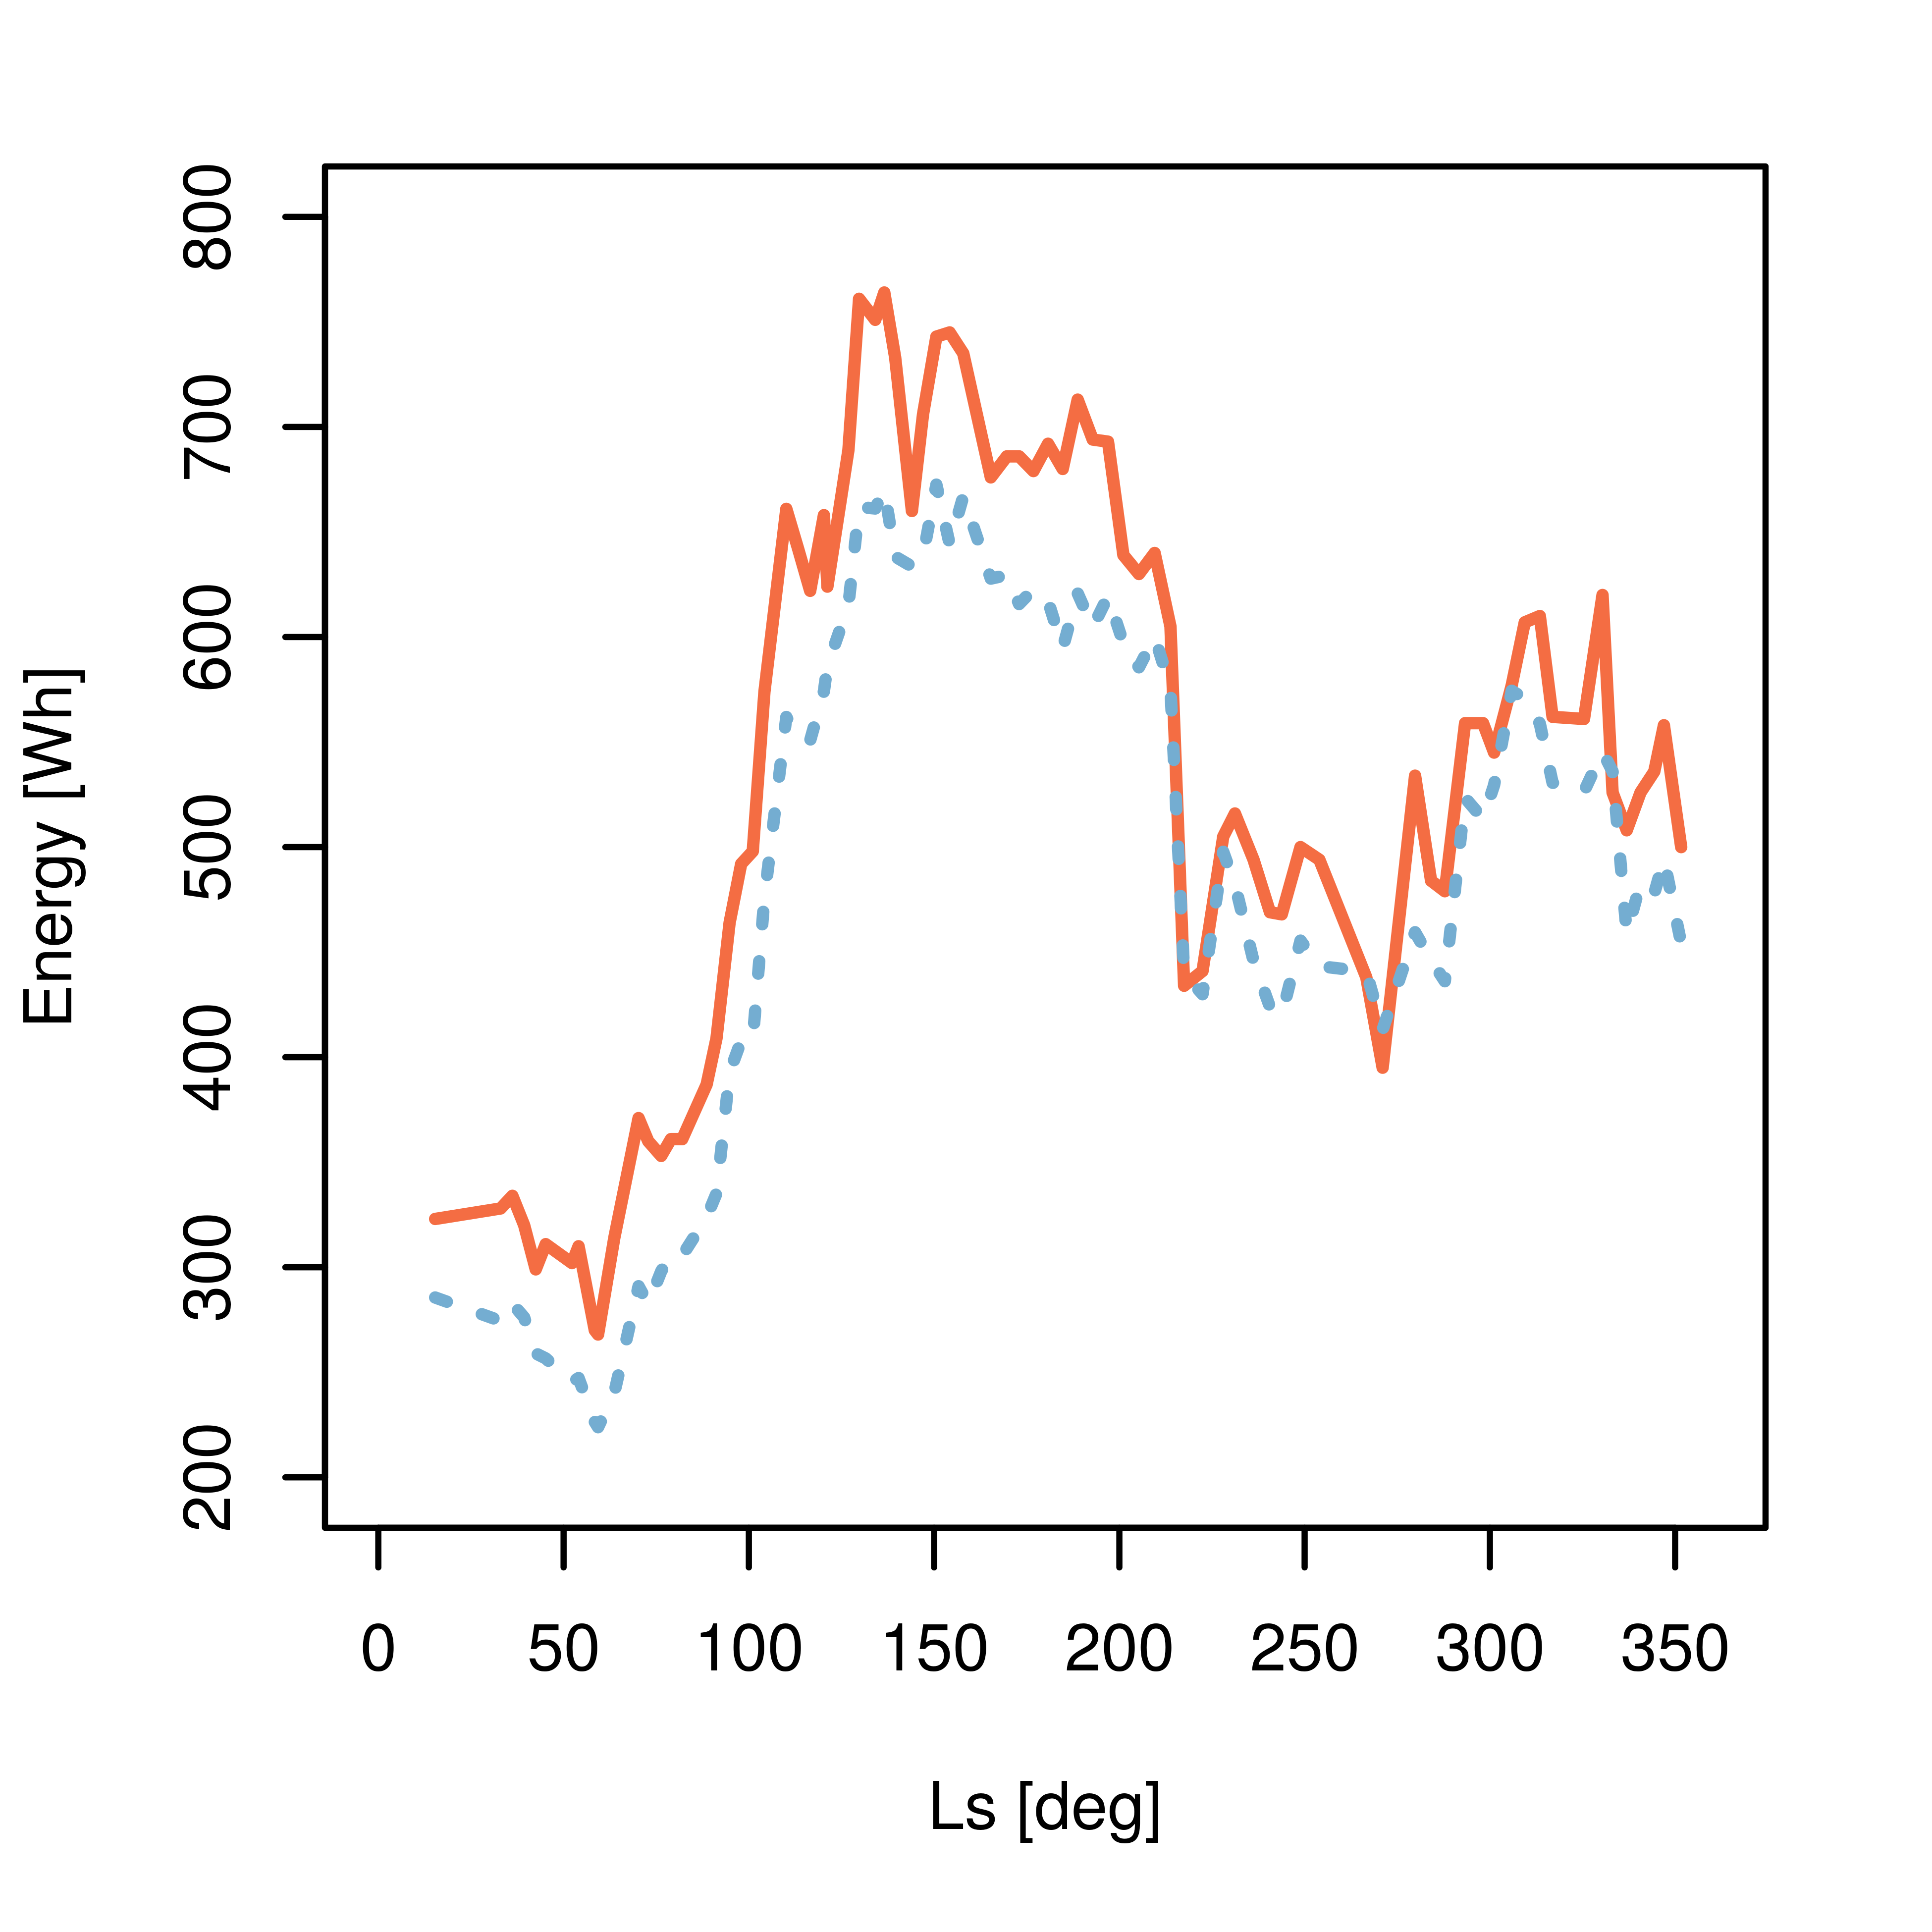
\includegraphics[height=\graphicsHeight]{sections/appendix/B/plots/predicted-vs-measured-energy-my32-adjusted.png}
		\subcaption{MY32}
		\label{fig:plot:sub:mer-energy-production-predicted-vs-reported-my32-adjusted}
	\end{subfigure}\\[0.8ex]
%% 2nd row
    \begin{subfigure}[t]{\subfigureWidth}
        \centering
		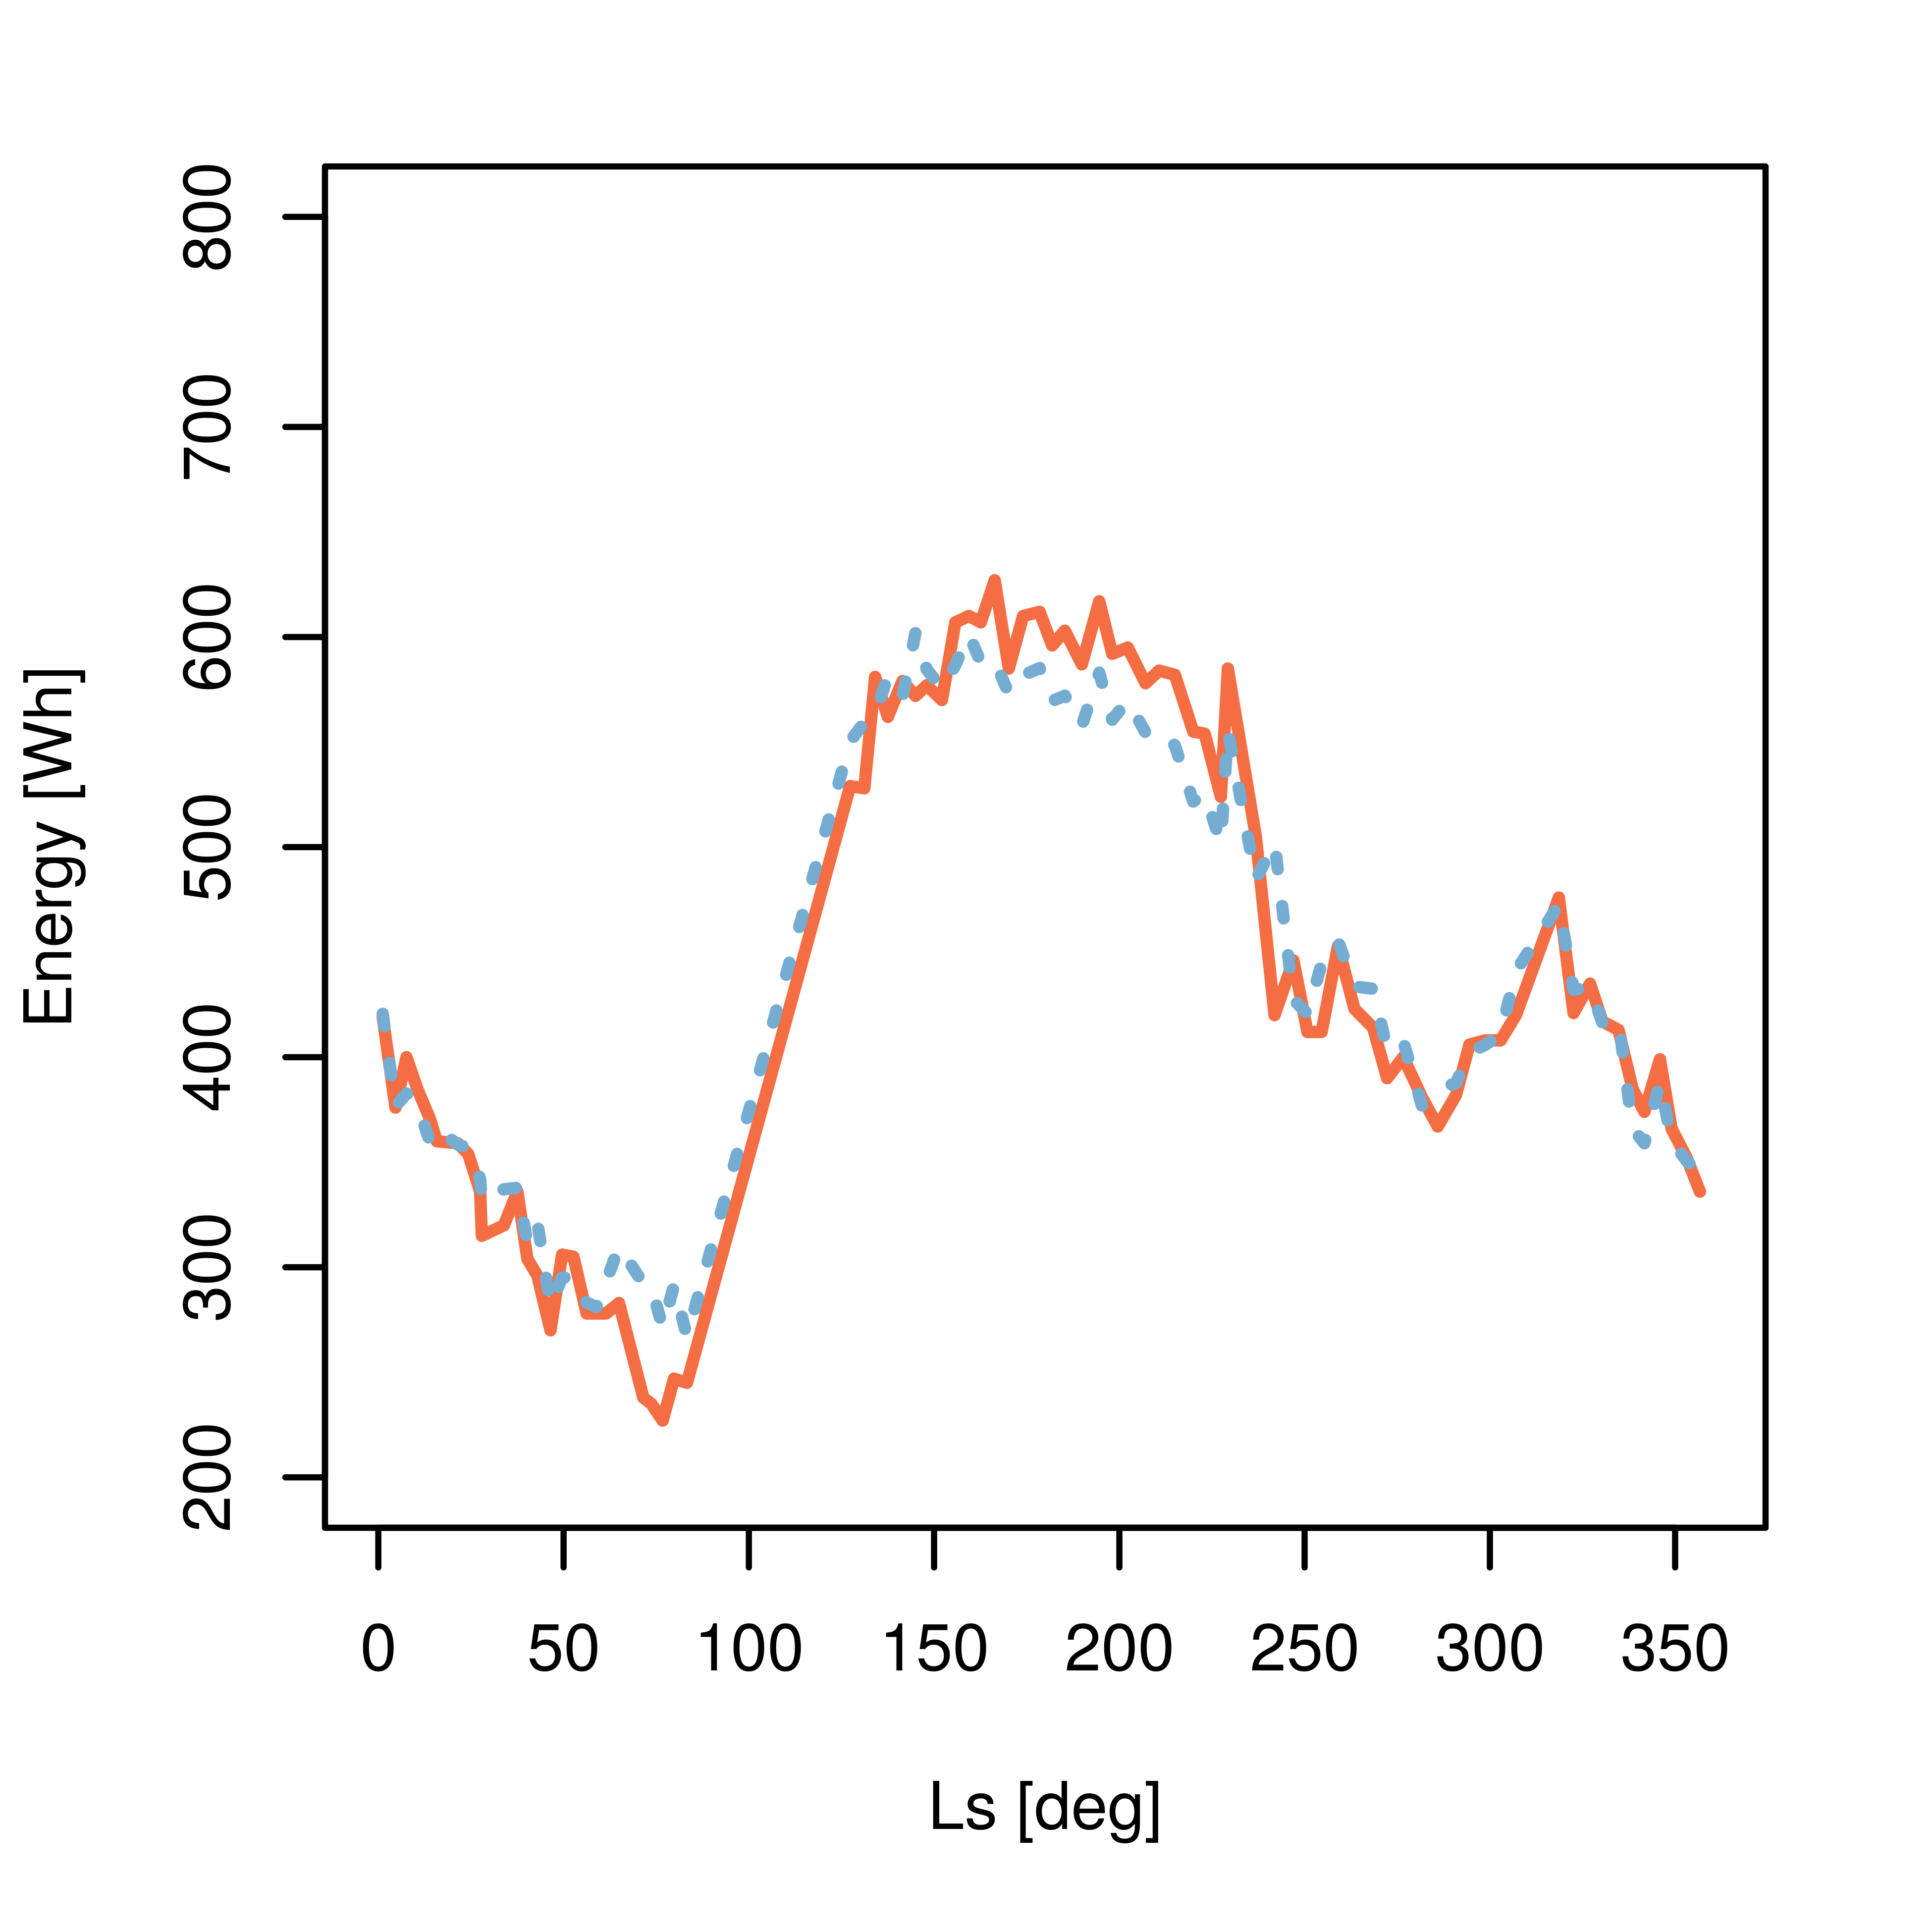
\includegraphics[height=\graphicsHeight]{sections/appendix/B/plots/predicted-vs-measured-energy-my29-adjusted-without-outliers.png}
		\subcaption{MY29}
		\label{fig:plot:sub:mer-energy-production-predicted-vs-reported-my29-adjusted-without-outliers}
	\end{subfigure}\hfill
	\begin{subfigure}[t]{\subfigureWidth}
        \centering
		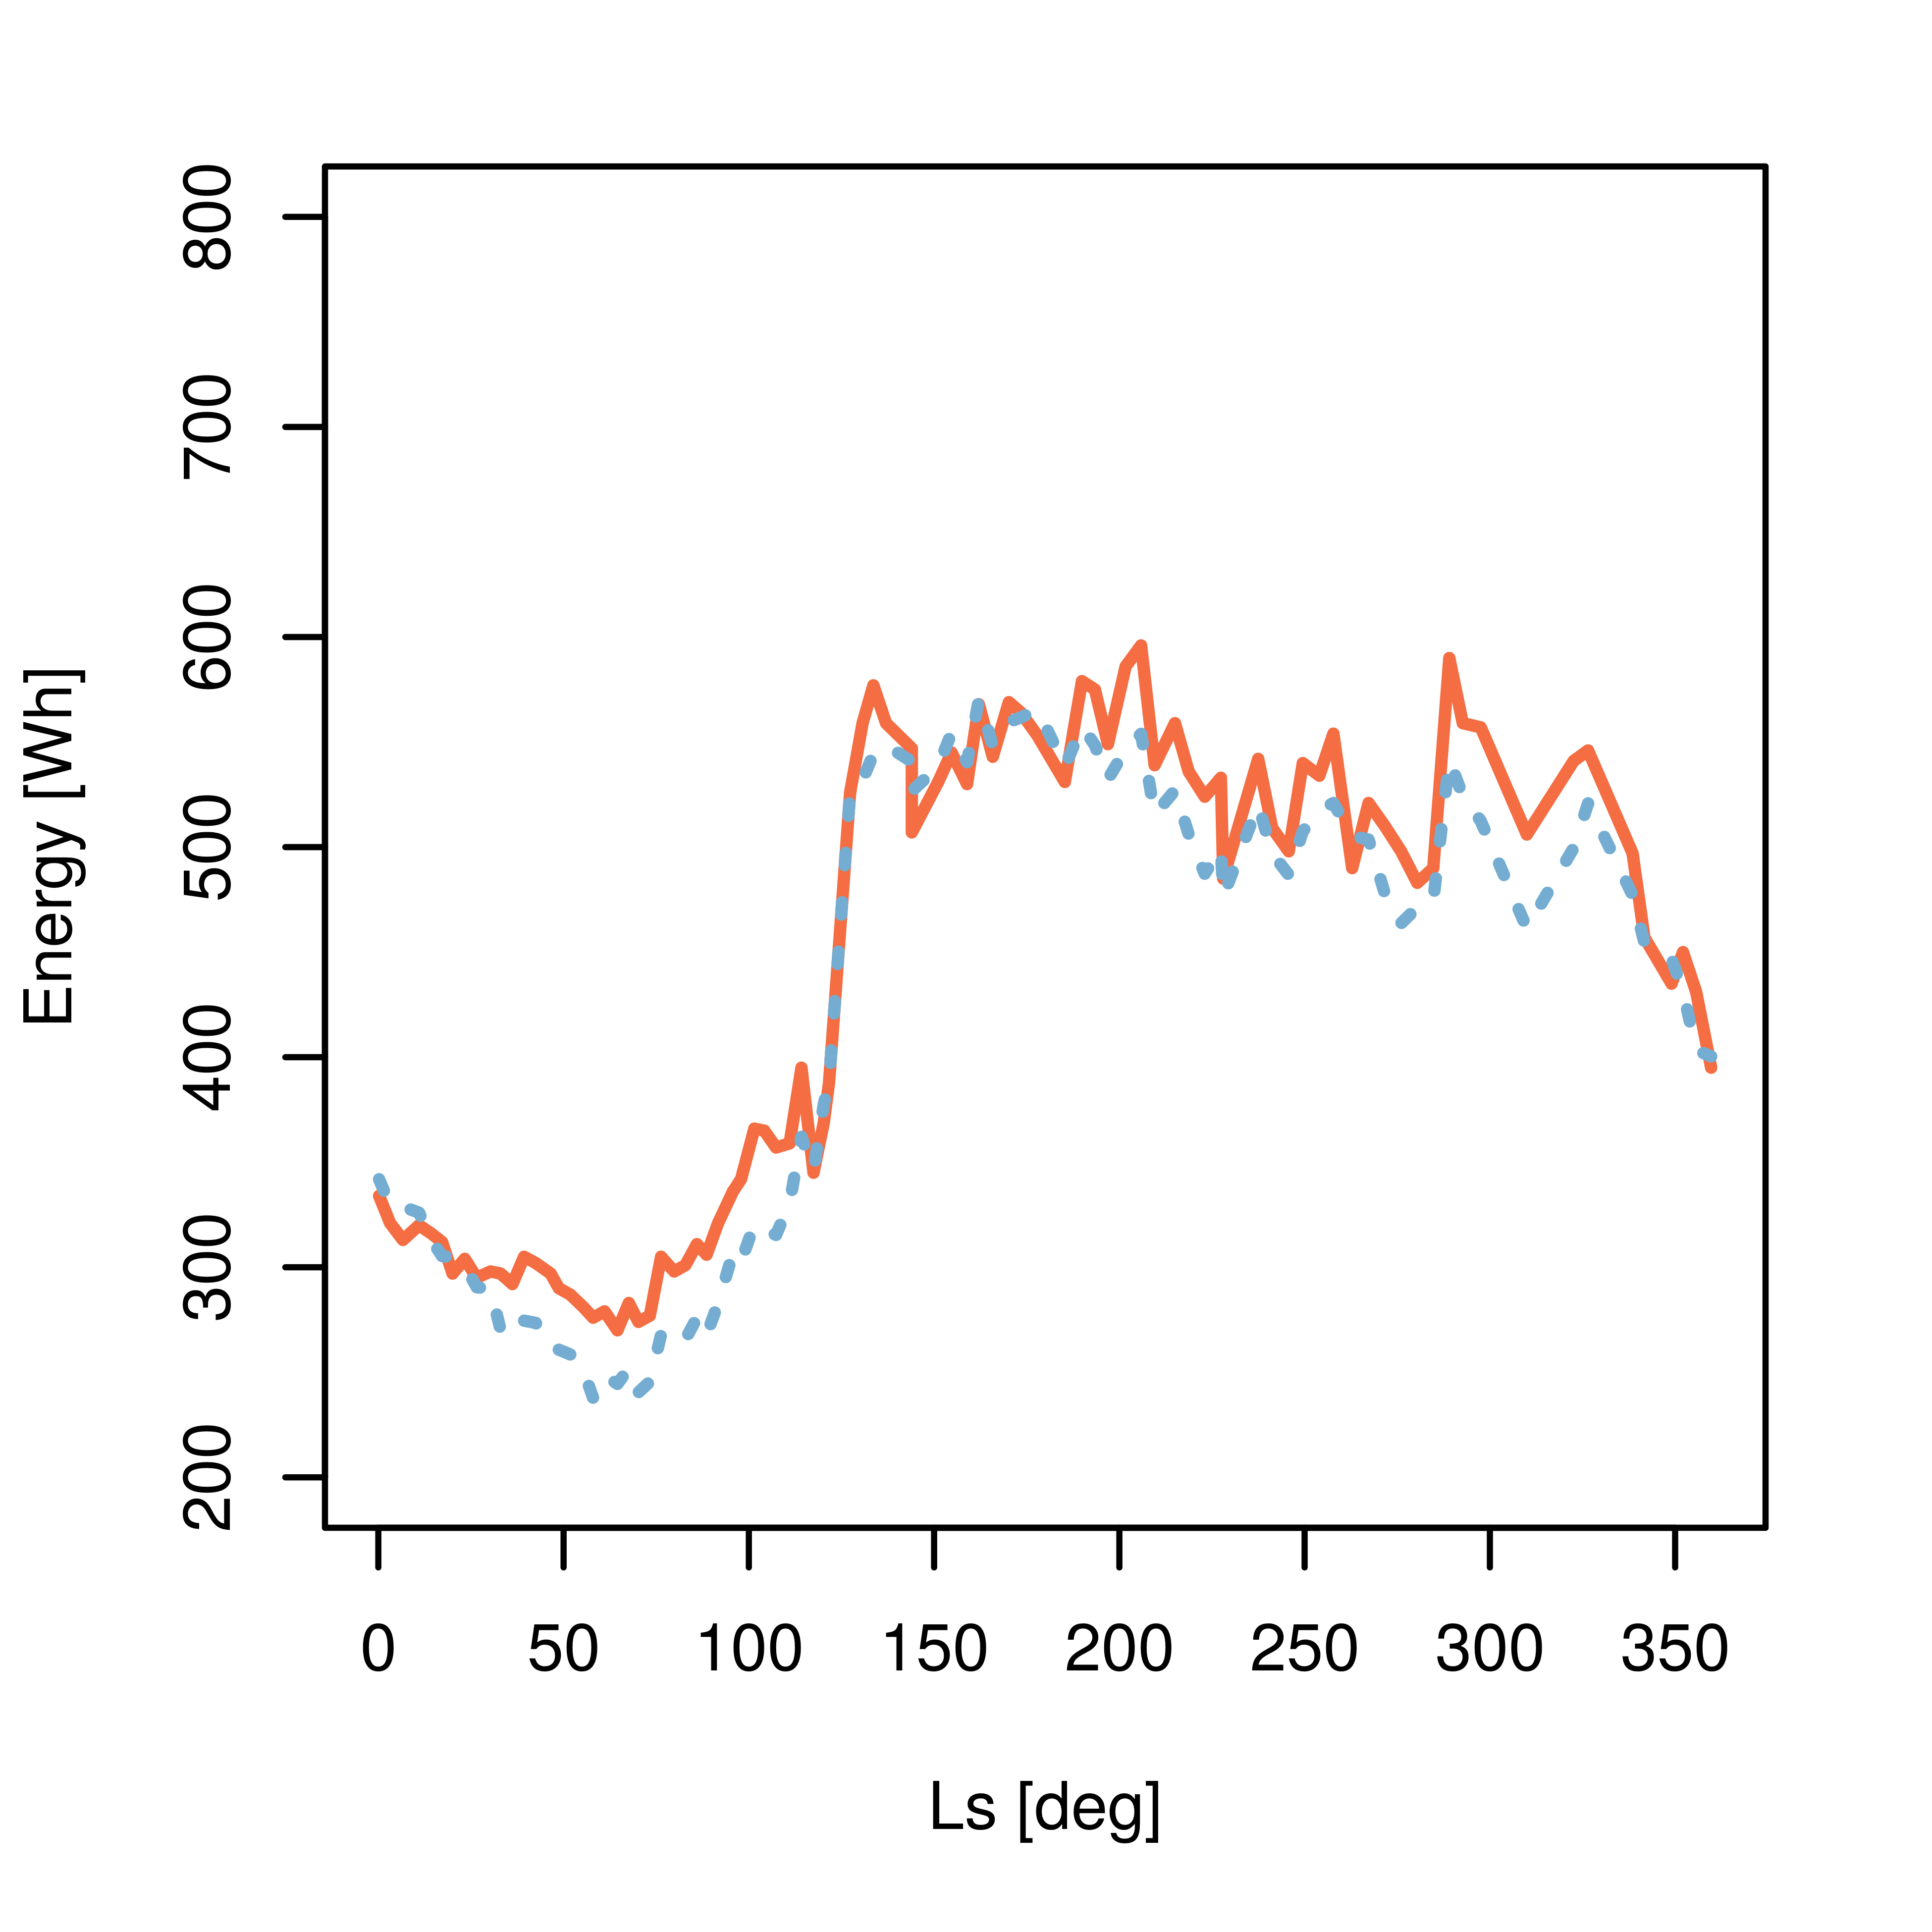
\includegraphics[height=\graphicsHeight]{sections/appendix/B/plots/predicted-vs-measured-energy-my30-adjusted-without-outliers.png}
		\subcaption{MY30}
		\label{fig:plot:sub:mer-energy-production-predicted-vs-reported-my30-adjusted-without-outliers}
	\end{subfigure}\hfill
    \begin{subfigure}[t]{\subfigureWidth}
        \centering
		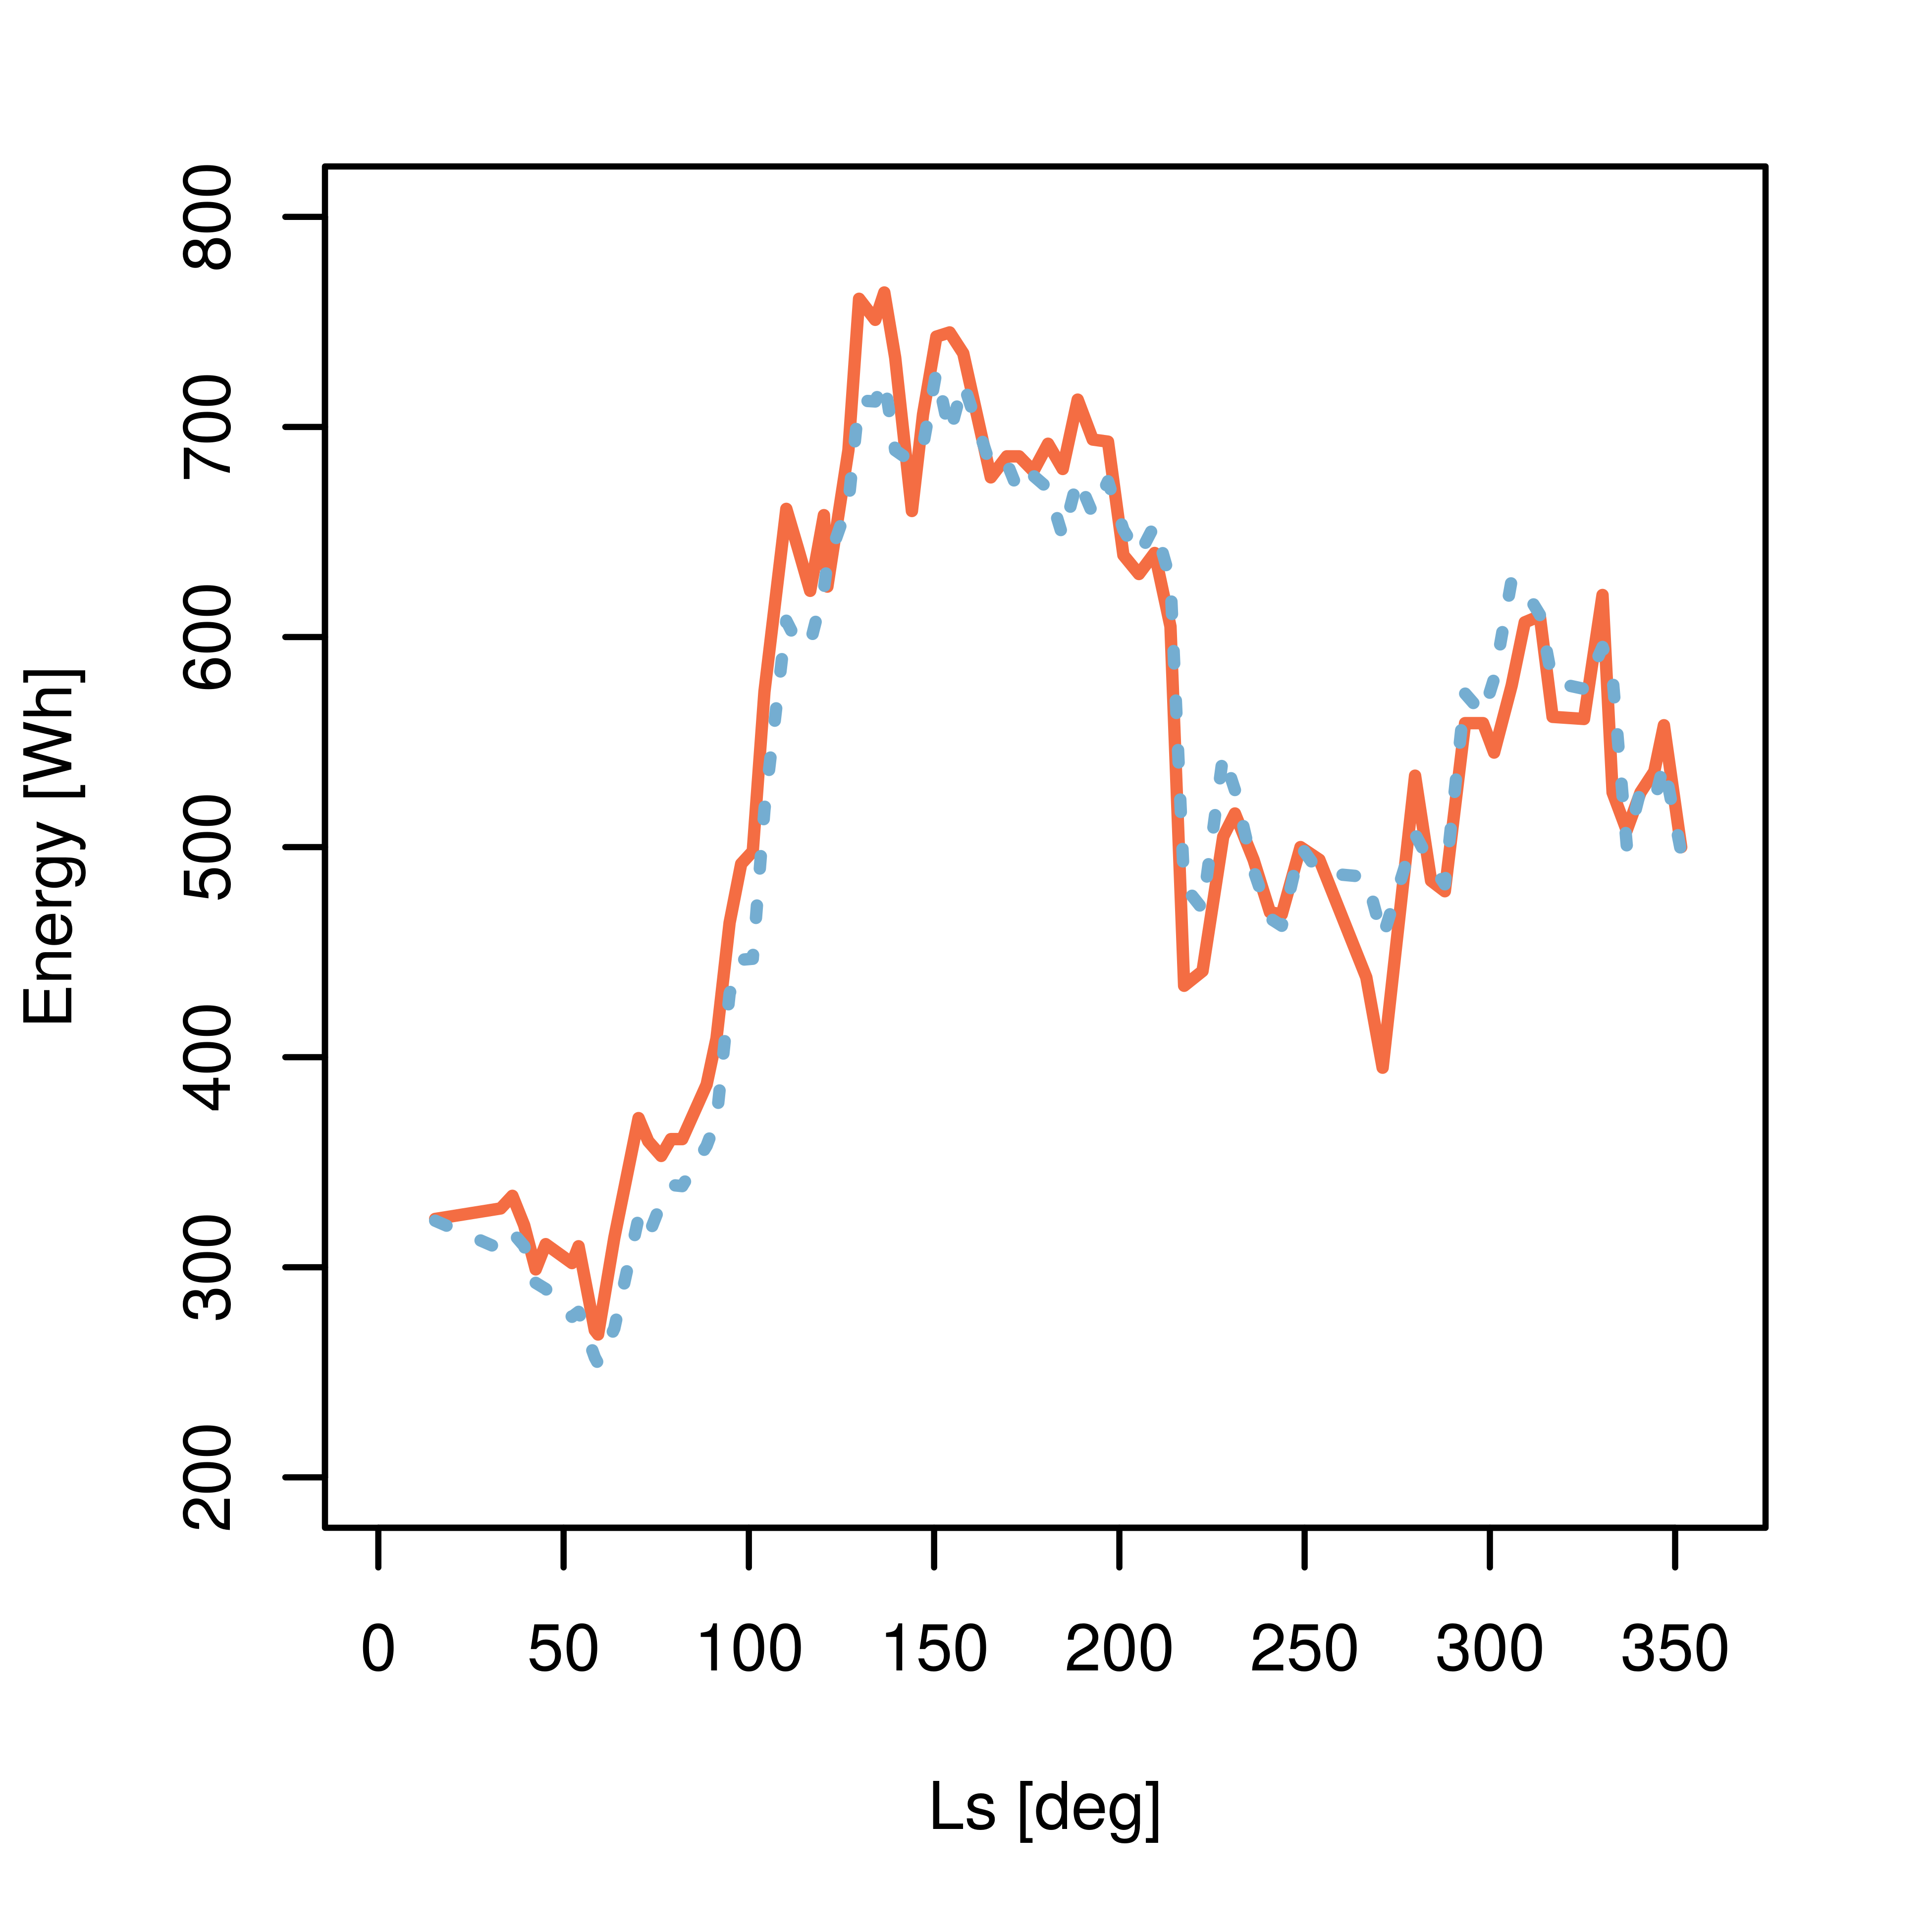
\includegraphics[height=\graphicsHeight]{sections/appendix/B/plots/predicted-vs-measured-energy-my32-adjusted-without-outliers.png}
		\subcaption{MY32}
		\label{fig:plot:sub:mer-energy-production-predicted-vs-reported-my32-adjusted-without-outliers}
	\end{subfigure}
    \caption[\ac{MER} Opportunity \ac{PV} energy production: adjusted prediction vs reported]
            {\ac{MER} Opportunity \ac{PV} energy production: adjusted prediction vs reported. The predicted lines across the first row were obtained with iteratively determined calculation adjustments that narrowed the calculated predicted values' error margin range from -33\%/+7\% to -10\%/+25\%. The second row was obtain in a similar fashion but with outlier divergences ignored which further narrowed the error margin range to -11\%/+5\%.}
    \label{fig:plot:mer-energy-production-predicted-vs-reported-adjusted-with-and-without-outliers}
\vspace{-2ex}
\end{figure}
